%!TEX root = ../../bug-taxo.tex

\subsection{How complex is each type of bugs?}

To answer {\bf RQ$_2$}, we analyze the complexity of each bug in terms of duplication, fixing time, comments, reopenning, files impacted, severity, changesets, hunks and chunks.

Figure \ref{fig:boxplots} presents nine boxplots describing our complexity metric for each type of each ecosystem.
In each sub-figure, the book plates are organized as follows: (a) Types 1 to 4 bugs for the Apache ecosystem, (b) Types 1 to 4 bugs for  the Netbeans ecosystem and (c) Types 1 to 4 bugs for both ecosystems combined.
For all the metrics, except the severity, the median is close to zero and we can observe many outliers.
Tables \ref{tab:apache-eco}, \ref{tab:netbeans-eco} and \ref{tab:overall-eco} present descriptive statistics about each metric for each type for the Apache ecosystem, the Netbeans ecosystem, and both ecosystems combined, respectively.
The descriptive statistics used are $\mu$:mean, $\sum$:sum, $\hat{x}$:median, $\sigma$:standard deviation and $\%$:percentage.
In addition, to the descriptive statistics, these tables present matrices of Mann-Whitney test for each metric and type.
We added the \checkmark~symbol to the Mann-Whitney tests results columns when the value is statistically significant (e.g. $\alpha \textless 0.05$) and \xmark~otherwise.

Finally, Table \ref{tab:chi-rq2} presents the Pearson's chi-squared test results for each complexity metric for Types 1 to 4 and our two types combination.
In what follows, we present our findings for each complexity metric.
Complexity metrics are divided into two groups: (a) process and (b) code metrics.
Process metrics refer to metrics that have been extracted from the project tracking system (i.e., fixing time, comments, reopening and severity).
Code metrics are directly computed using the source code used to fix a given bug (i.e., files impacted, changesets required, hunks and chunks).
We acknowledge that these complexity metrics only represent an abstraction of the actual complexity of a given bug as they cannot account for the actual thought process and expertise required to craft a fix.
However, we believe that they are an accurate abstraction. Moreover, they are used in several studies in the field to  approximate the complexity of a bug \cite{Weiß2007,Saha2014,Nam2013,Anvik2006,Nagappan}.

\begin{figure*}
\centering
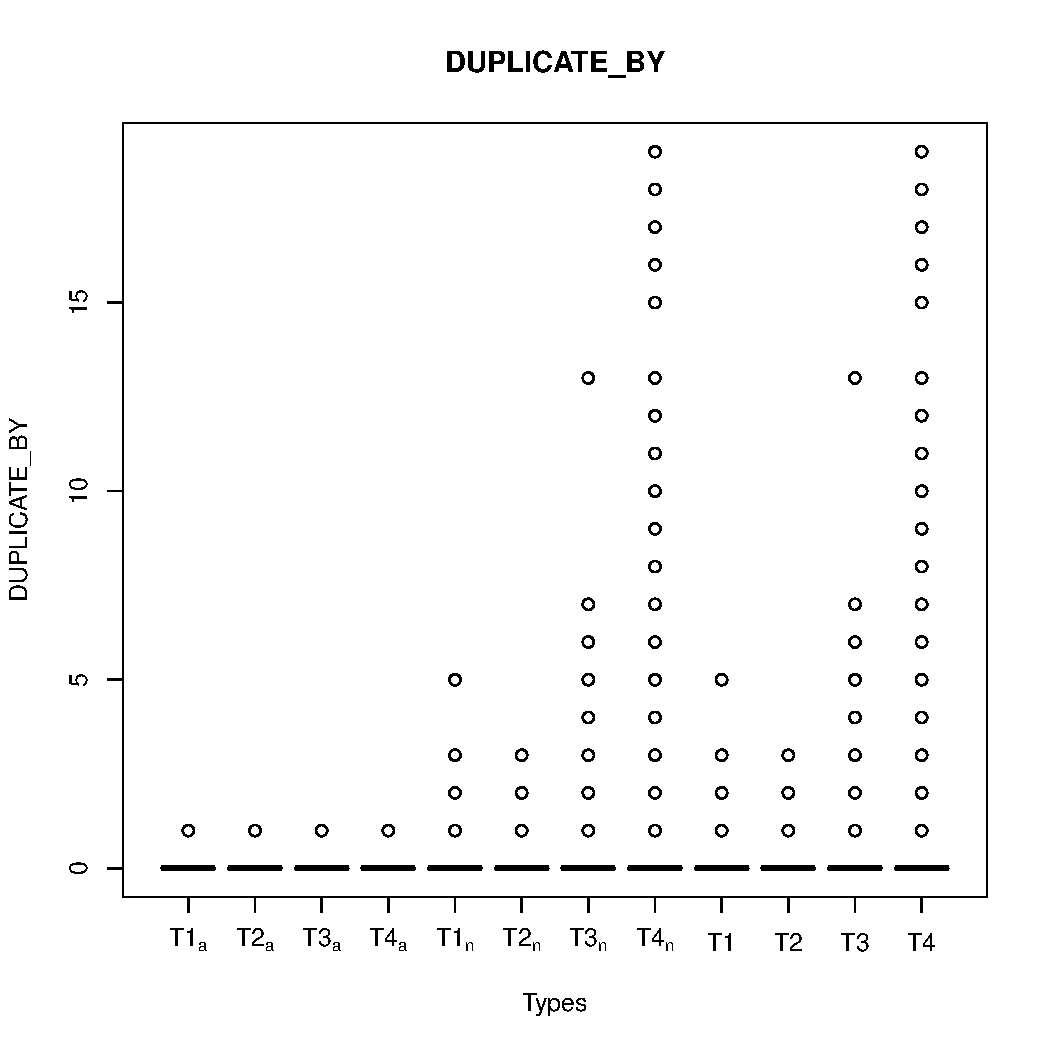
\includegraphics[page=1, width=0.45\textwidth]{extract/Rplots}
\includegraphics[page=2, width=0.45\textwidth]{extract/Rplots} \\
\includegraphics[page=3, width=0.45\textwidth]{extract/Rplots}
\includegraphics[page=4, width=0.45\textwidth]{extract/Rplots} \\
\includegraphics[page=5, width=0.45\textwidth]{extract/Rplots}
\includegraphics[page=6, width=0.45\textwidth]{extract/Rplots}

\label{fig:boxplots}}

\end{figure*}

\begin{figure*}
\centering
\includegraphics[page=7, width=0.45\textwidth]{extract/Rplots}
\includegraphics[page=8, width=0.45\textwidth]{extract/Rplots} \\
\includegraphics[page=9, width=0.45\textwidth]{extract/Rplots}

\caption{Complexity metrics boxplots. From left to right and top to bottom: Duplicate, Fixing time, Comments, Reopening, Files impacted, Severity, Changesets, Hunks and Chunks.
\label{fig:boxplots}}

\end{figure*}

%!TEX root = ..bug-taxo.tex

% Please add the following required packages to your document preamble:
% \usepackage{graphicx}
\begin{table*}[]
\centering
\samll
\setlength\extrarowheight{6pt}
\caption{My caption}
\label{my-label}
\begin{tabular}{ccccccc|ccccc}

Types & Metric &$^\mu$ & $^\sum$ & $^\hat{x}$ & $^\sigma$ & $^\%$ & T1 & T2 & T3 & T4 \\ \hline \rowcolor{gray!25}
& Dup. & 0.026 & 51 & 0 & 0.2 & 14.8 & n.a & \xmark (0.53) & \checkmark  (\textless 0.05) & \xmark (0.45)  \\ \rowcolor{gray!25}
& Tim. & 91.574 & 180217 & 4 & 262 & 21.8 & n.a & \checkmark  (\textless 0.05) & \checkmark  (\textless 0.05) & \checkmark  (\textless 0.05)  \\ \rowcolor{gray!25}
& Com. & 4.355 & 8571 & 3 & 4.7 & 9.5 & n.a & \checkmark  (\textless 0.05) & \xmark (0.17) & \checkmark  (\textless 0.05)  \\ \rowcolor{gray!25}
& Reo. & 0.062 & 122 & 0 & 0.3 & 13.8 & n.a & \xmark (0.29) & \checkmark  (\textless 0.05) & \checkmark  (\textless 0.05)  \\ \rowcolor{gray!25}
T1 & Fil. & 0.991 & 1950 & 1 & 0.1 & 3.7 & n.a & \checkmark  (\textless 0.05) & \xmark (0.28) & \checkmark  (\textless 0.05)  \\ \rowcolor{gray!25}
& Sev. & 3.423 & 6737 & 4 & 1.3 & 13.2 & n.a & \xmark (0.18) & \checkmark  (\textless 0.05) & \checkmark  (\textless 0.05)  \\ \rowcolor{gray!25}
& Cha. & 1 & 1968 & 1 & 0 & 1.9 & n.a & \checkmark  (\textless 0.05) & \checkmark  (\textless 0.05) & \checkmark  (\textless 0.05)  \\ \rowcolor{gray!25}
& Hun. & 3.814 & 7506 & 3 & 2.4 & 0 & n.a & \checkmark  (\textless 0.05) & \checkmark  (\textless 0.05) & \checkmark  (\textless 0.05)  \\ \rowcolor{gray!25}
& Chur. & 18.761 & 36921 & 7 & 48.6 & 0 & n.a & \checkmark  (\textless 0.05) & \xmark (0.09) & \checkmark  (\textless 0.05)  \\


 & Dup. & 0.022 & 28 & 0 & 0.1 & 8.1 & \xmark (0.53) & n.a & \xmark (0.16) & \xmark (0.19)  \\
 & Tim. & 115.158 & 143717 & 8 & 294.1 & 17.4 & \checkmark  (\textless 0.05) & n.a & \checkmark  (\textless 0.05) & \checkmark  (\textless 0.05)  \\
 & Com. & 5.041 & 6291 & 4 & 4.7 & 7 & \checkmark  (\textless 0.05) & n.a & \checkmark  (\textless 0.05) & \checkmark  (\textless 0.05)  \\
 & Reo. & 0.071 & 89 & 0 & 0.3 & 10.1 & \xmark (0.29) & n.a & \checkmark  (\textless 0.05) & \xmark (0.59)  \\
T2 & Fil. & 4.381 & 5468 & 2 & 20.4 & 10.5 & \checkmark  (\textless 0.05) & n.a & \checkmark  (\textless 0.05) & \checkmark  (\textless 0.05)  \\
 & Sev. & 3.498 & 4365 & 4 & 1.2 & 8.6 & \xmark (0.18) & n.a & \checkmark  (\textless 0.05) & \checkmark  (\textless 0.05)  \\
 & Cha. & 4.681 & 5842 & 2 & 20.4 & 5.5 & \checkmark  (\textless 0.05) & n.a & \checkmark  (\textless 0.05) & \checkmark  (\textless 0.05)  \\
 & Hun. & 561.995 & 701370 & 14 & 13628.2 & 3.9 & \checkmark  (\textless 0.05) & n.a & \checkmark  (\textless 0.05) & \checkmark  (\textless 0.05)  \\
 & Chur. & 14184.869 & 17702716 & 88 & 400710.2 & 8 & \checkmark  (\textless 0.05) & n.a & \checkmark  (\textless 0.05) & \checkmark  (\textless 0.05)  \\

 \rowcolor{gray!25}
 & Dup. & 0.016 & 50 & 0 & 0.1 & 14.5 & \checkmark  (\textless 0.05) & \xmark (0.16) & n.a & \checkmark  (\textless 0.05)  \\ \rowcolor{gray!25}
 & Tim. & 35.892 & 111300 & 1 & 151.8 & 13.5 & \checkmark  (\textless 0.05) & \checkmark  (\textless 0.05) & n.a & \checkmark  (\textless 0.05)  \\ \rowcolor{gray!25}
 & Com. & 4.422 & 13712 & 3 & 4.4 & 15.2 & \xmark (0.17) & \checkmark  (\textless 0.05) & n.a & \checkmark  (\textless 0.05)  \\ \rowcolor{gray!25}
 & Reo. & 0.033 & 101 & 0 & 0.2 & 11.5 & \checkmark  (\textless 0.05) & \checkmark  (\textless 0.05) & n.a & \checkmark  (\textless 0.05)  \\ \rowcolor{gray!25}
 T3 & Fil. & 0.994 & 3081 & 1 & 0.1 & 5.9 & \xmark (0.28) & \checkmark  (\textless 0.05) & n.a & \checkmark  (\textless 0.05)  \\ \rowcolor{gray!25}
 & Sev. & 3.644 & 11300 & 4 & 1.1 & 22.2 & \checkmark  (\textless 0.05) & \checkmark  (\textless 0.05) & n.a & \checkmark  (\textless 0.05)  \\ \rowcolor{gray!25}
 & Cha. & 1 & 3101 & 1 & 0 & 2.9 & \checkmark  (\textless 0.05) & \checkmark  (\textless 0.05) & n.a & \checkmark  (\textless 0.05)  \\ \rowcolor{gray!25}
 & Hun. & 4.022 & 12472 & 3 & 3.4 & 0.1 & \checkmark  (\textless 0.05) & \checkmark  (\textless 0.05) & n.a & \checkmark  (\textless 0.05)  \\ \rowcolor{gray!25}
 & Chur. & 16.954 & 52573 & 6 & 49.8 & 0 & \xmark (0.09) & \checkmark  (\textless 0.05) & n.a & \checkmark  (\textless 0.05)  \\


& Dup. & 0.029 & 216 & 0 & 0.2 & 62.6 & \xmark (0.45) & \xmark (0.19) & \checkmark  (\textless 0.05) & n.a  \\
& Tim. & 52.76 & 391586 & 4 & 182.2 & 47.4 & \checkmark  (\textless 0.05) & \checkmark  (\textless 0.05) & \checkmark  (\textless 0.05) & n.a  \\
& Com. & 8.313 & 61701 & 5 & 10.2 & 68.3 & \checkmark  (\textless 0.05) & \checkmark  (\textless 0.05) & \checkmark  (\textless 0.05) & n.a  \\
& Reo. & 0.077 & 570 & 0 & 0.3 & 64.6 & \checkmark  (\textless 0.05) & \xmark (0.59) & \checkmark  (\textless 0.05) & n.a  \\
T4 & Fil. & 5.633 & 41805 & 3 & 14 & 79.9 & \checkmark  (\textless 0.05) & \checkmark  (\textless 0.05) & \checkmark  (\textless 0.05) & n.a  \\
& Sev. & 3.835 & 28466 & 4 & 1 & 56 & \checkmark  (\textless 0.05) & \checkmark  (\textless 0.05) & \checkmark  (\textless 0.05) & n.a  \\
& Cha. & 12.861 & 95455 & 4 & 52.2 & 89.7 & \checkmark  (\textless 0.05) & \checkmark  (\textless 0.05) & \checkmark  (\textless 0.05) & n.a  \\
& Hun. & 2305.868 & 17114149 & 30 & 58094.7 & 96 & \checkmark  (\textless 0.05) & \checkmark  (\textless 0.05) & \checkmark  (\textless 0.05) & n.a  \\
& Chur. & 27249.773 & 202247816 & 204 & 320023.5 & 91.9 & \checkmark  (\textless 0.05) & \checkmark  (\textless 0.05) & \checkmark  (\textless 0.05) & n.a

\end{tabular}%
\end{table*}

%!TEX root = ..bug-taxo.tex

\begin{table*}[]
\centering
\small
\setlength\extrarowheight{6pt}
\caption{My caption}
\label{my-label}
\begin{tabular}{ccccccc|ccccc}

Types & Metric &$^\mu$ & $^\sum$ & $^\hat{x}$ & $^\sigma$ & $^\%$ & T1 & T2 & T3 & T4 \\ \hline \rowcolor{gray!25}

& Dup. & 0.086 & 67 & 0 & 0.4 & 2.5 & n.a & \xmark (0.39) & \xmark (0.24) & \xmark (0.86) \\  \rowcolor{gray!25}
& Tim. & 92.759 & 71981 & 10 & 219.1 & 2.3 & n.a & \checkmark  (\textless 0.05) & \xmark (0.15) & \checkmark  (\textless 0.05) \\  \rowcolor{gray!25}
& Com. & 4.687 & 3637 & 3 & 4.1 & 2.4 & n.a & \checkmark  (\textless 0.05) & \xmark (0.83) & \checkmark  (\textless 0.05)  \\  \rowcolor{gray!25}
& Reo. & 0.054 & 42 & 0 & 0.3 & 1.9 & n.a & \xmark (0.1) & \xmark (0.58) & \checkmark  (\textless 0.05)  \\  \rowcolor{gray!25}
T1 & Fil. & 1.735 & 1346 & 1 & 13.2 & 0.8 & n.a & \checkmark  (\textless 0.05) & \checkmark  (\textless 0.05) & \checkmark  (\textless 0.05)  \\  \rowcolor{gray!25}
& Sev. & 4.314 & 3348 & 3 & 1.5 & 3.1 & n.a & \xmark (0.66) & \checkmark  (\textless 0.05) & \checkmark  (\textless 0.05)  \\  \rowcolor{gray!25}
& Cha. & 1.085 & 842 & 1 & 0.4 & 2 & n.a & \xmark (0.99) & \xmark (0.26) & \checkmark  (\textless 0.05)  \\  \rowcolor{gray!25}
& Hun. & 4.405 & 3418 & 3 & 7 & 0.5 & n.a & \checkmark  (\textless 0.05) & \xmark (0.13) & \checkmark  (\textless 0.05)  \\  \rowcolor{gray!25}
& Chur. & 5.089 & 3949 & 2 & 12.5 & 0.3 & n.a & \checkmark  (\textless 0.05) & \checkmark  (\textless 0.05) & \checkmark  (\textless 0.05)  \\


 & Dup. & 0.067 & 16 & 0 & 0.3 & 0.6 & \xmark (0.39) & n.a & \xmark (0.73) & \xmark (0.39) \\
 & Tim. & 111.9 & 26856 & 16 & 308.6 & 0.9 & \checkmark  (\textless 0.05) & n.a & \checkmark  (\textless 0.05) & \xmark (0.41) \\
 & Com. & 4.433 & 1064 & 3 & 4 & 0.7 & \checkmark  (\textless 0.05) & n.a & \checkmark  (\textless 0.05) & \checkmark  (\textless 0.05) \\
 & Reo. & 0.079 & 19 & 0 & 0.3 & 0.9 & \xmark (0.1) & n.a & \xmark (0.11) & \xmark (0.97) \\
T2 & Fil. & 8.804 & 2113 & 2 & 42.7 & 1.3 & \checkmark  (\textless 0.05) & n.a & \checkmark  (\textless 0.05) & \checkmark  (\textless 0.05) \\
 & Sev. & 4.362 & 1047 & 3 & 1.5 & 1 & \xmark (0.66) & n.a & \checkmark  (\textless 0.05) & \checkmark  (\textless 0.05) \\
 & Cha. & 1.075 & 258 & 1 & 0.3 & 0.6 & \xmark (0.99) & n.a & \xmark (0.5) & \checkmark  (\textless 0.05)  \\
 & Hun. & 21.887 & 5253 & 8 & 62.7 & 0.7 & \checkmark  (\textless 0.05) & n.a & \checkmark  (\textless 0.05) & \checkmark  (\textless 0.05) \\
 & Chur. & 32.263 & 7743 & 8 & 125.8 & 0.7 & \checkmark  (\textless 0.05) & n.a & \checkmark  (\textless 0.05) & \checkmark  (\textless 0.05)  \\

 \rowcolor{gray!25}
& Dup. & 0.074 & 620 & 0 & 0.4 & 23.3 & \xmark (0.24) & \xmark (0.73) & n.a & \checkmark  (\textless 0.05)  \\  \rowcolor{gray!25}
& Tim. & 87.033 & 728642 & 9 & 233.6 & 23.8 & \xmark (0.15) & \checkmark  (\textless 0.05) & n.a & \checkmark  (\textless 0.05) \\  \rowcolor{gray!25}
& Com. & 4.73 & 39599 & 3 & 4.3 & 26.5 & \xmark (0.83) & \checkmark  (\textless 0.05) & n.a & \checkmark  (\textless 0.05)  \\  \rowcolor{gray!25}
& Reo. & 0.06 & 499 & 0 & 0.3 & 22.7 & \xmark (0.58) & \xmark (0.11) & n.a & \checkmark  (\textless 0.05)  \\  \rowcolor{gray!25}
T3 & Fil. & 1.306 & 10932 & 1 & 5.1 & 6.8 & \checkmark  (\textless 0.05) & \checkmark  (\textless 0.05) & n.a & \checkmark  (\textless 0.05) \\  \rowcolor{gray!25}
& Sev. & 4.021 & 33666 & 3 & 1.4 & 31.4 & \checkmark  (\textless 0.05) & \checkmark  (\textless 0.05) & n.a & \checkmark  (\textless 0.05) \\  \rowcolor{gray!25}
& Cha. & 1.065 & 8917 & 1 & 0.3 & 21 & \xmark (0.26) & \xmark (0.5) & n.a & \checkmark  (\textless 0.05) \\  \rowcolor{gray!25}
& Hun. & 5.15 & 43115 & 3 & 12.4 & 5.8 & \xmark (0.13) & \checkmark  (\textless 0.05) & n.a & \checkmark  (\textless 0.05) \\  \rowcolor{gray!25}
& Chur. & 6.727 & 56317 & 2 & 22 & 4.9 & \checkmark  (\textless 0.05) & \checkmark  (\textless 0.05) & n.a & \checkmark  (\textless 0.05)  \\


 & Dup. & 0.113 & 1959 & 0 & 0.7 & 73.6 & \xmark (0.86) & \xmark (0.39) & \checkmark  (\textless 0.05) & n.a \\
 & Tim. & 128.833 & 2237319 & 13 & 332.8 & 73 & \checkmark  (\textless 0.05) & \xmark (0.41) & \checkmark  (\textless 0.05) & n.a \\
 & Com. & 6.058 & 105202 & 4 & 6.7 & 70.4 & \checkmark  (\textless 0.05) & \checkmark  (\textless 0.05) & \checkmark  (\textless 0.05) & n.a \\
 & Reo. & 0.094 & 1639 & 0 & 0.4 & 74.5 & \checkmark  (\textless 0.05) & \xmark (0.97) & \checkmark  (\textless 0.05) & n.a & \\
T4 & Fil. & 8.408 & 146019 & 4 & 25.1 & 91 & \checkmark  (\textless 0.05) & \checkmark  (\textless 0.05) & \checkmark  (\textless 0.05) & n.a \\
 & Sev. & 3.982 & 69159 & 3 & 1.4 & 64.5 & \checkmark  (\textless 0.05) & \checkmark  (\textless 0.05) & \checkmark  (\textless 0.05) & n.a \\
 & Cha. & 1.871 & 32494 & 2 & 1.2 & 76.4 & \checkmark  (\textless 0.05) & \checkmark  (\textless 0.05) & \checkmark  (\textless 0.05) & n.a \\
 & Hun. & 40.195 & 698022 & 13 & 98.3 & 93.1 & \checkmark  (\textless 0.05) & \checkmark  (\textless 0.05) & \checkmark  (\textless 0.05) & n.a  \\
 & Chur. & 61.893 & 1074830 & 15 & 178.6 & 94 & \checkmark  (\textless 0.05) & \checkmark  (\textless 0.05) & \checkmark  (\textless 0.05) & n.a

\end{tabular}%
\end{table*}

%!TEX root = ..bug-taxo.tex

\begin{table*}[]
\centering
\samll
\setlength\extrarowheight{6pt}
\caption{My caption}
\label{my-label}
\begin{tabular}{ccccccc|ccccc}

Types & Metric &$^\mu$ & $^\sum$ & $^\hat{x}$ & $^\sigma$ & $^\%$ & T1 & T2 & T3 & T4 \\ \hline \rowcolor{gray!25}
& Dup. & 0.043 & 118 & 0 & 0.3 & 3.9 & n.a & \xmark (0.09) & \xmark (0.16) & \checkmark  (\textless 0.05)  \\  \rowcolor{gray!25}
& Tim. & 91.909 & 252198 & 6 & 250.6 & 6.5 & n.a & \checkmark  (\textless 0.05) & \checkmark  (\textless 0.05) & \checkmark  (\textless 0.05)  \\  \rowcolor{gray!25}
& Com. & 4.449 & 12208 & 3 & 4.5 & 5.1 & n.a & \checkmark  (\textless 0.05) & \checkmark  (\textless 0.05) & \checkmark  (\textless 0.05)  \\  \rowcolor{gray!25}
& Reo. & 0.06 & 164 & 0 & 0.3 & 5.3 & n.a & \xmark (0.07) & \checkmark  (\textless 0.05) & \checkmark  (\textless 0.05)  \\  \rowcolor{gray!25}
T1 & Fil. & 1.201 & 3296 & 1 & 7 & 1.5 & n.a & \checkmark  (\textless 0.05) & \checkmark  (\textless 0.05) & \checkmark  (\textless 0.05)  \\  \rowcolor{gray!25}
& Sev. & 3.675 & 10085 & 4 & 1.4 & 6.4 & n.a & \xmark (0.97) & \xmark (0.17) & \checkmark  (\textless 0.05)  \\  \rowcolor{gray!25}
& Cha. & 1.024 & 2810 & 1 & 0.2 & 1.9 & n.a & \checkmark  (\textless 0.05) & \checkmark  (\textless 0.05) & \checkmark  (\textless 0.05)  \\  \rowcolor{gray!25}
& Hun. & 3.981 & 10924 & 3 & 4.3 & 0.1 & n.a & \checkmark  (\textless 0.05) & \checkmark  (\textless 0.05) & \checkmark  (\textless 0.05)  \\  \rowcolor{gray!25}
& Chur. & 14.894 & 40870 & 5 & 42.2 & 0 & n.a & \checkmark  (\textless 0.05) & \checkmark  (\textless 0.05) & \checkmark  (\textless 0.05)  \\


& Dup. & 0.03 & 44 & 0 & 0.2 & 1.5 & \xmark (0.09) & n.a & \checkmark  (\textless 0.05) & \checkmark  (\textless 0.05)  \\
& Tim. & 114.632 & 170573 & 9 & 296.4 & 4.4 & \checkmark  (\textless 0.05) & n.a & \checkmark  (\textless 0.05) & \xmark (0.15)  \\
& Com. & 4.943 & 7355 & 3 & 4.6 & 3.1 & \checkmark  (\textless 0.05) & n.a & \xmark (0.72) & \checkmark  (\textless 0.05)  \\
& Reo. & 0.073 & 108 & 0 & 0.3 & 3.5 & \xmark (0.07) & n.a & \checkmark  (\textless 0.05) & \xmark (0.47)  \\
T2 & Fil. & 5.095 & 7581 & 2 & 25.4 & 3.6 & \checkmark  (\textless 0.05) & n.a & \checkmark  (\textless 0.05) & \checkmark  (\textless 0.05)  \\
& Sev. & 3.637 & 5412 & 4 & 1.3 & 3.4 & \xmark (0.97) & n.a & \xmark (0.44) & \xmark (0.1)  \\
& Cha. & 4.099 & 6100 & 2 & 18.7 & 4.1 & \checkmark  (\textless 0.05) & n.a & \checkmark  (\textless 0.05) & \checkmark  (\textless 0.05)  \\
& Hun. & 474.881 & 706623 & 12 & 12481.7 & 3.8 & \checkmark  (\textless 0.05) & n.a & \checkmark  (\textless 0.05) & \checkmark  (\textless 0.05)  \\
& Chur. & 11902.19 & 17710459 & 62 & 366988 & 8 & \checkmark  (\textless 0.05) & n.a & \checkmark  (\textless 0.05) & \checkmark  (\textless 0.05)  \\

 \rowcolor{gray!25}
& Dup. & 0.058 & 670 & 0 & 0.4 & 22.3 & \xmark (0.16) & \checkmark  (\textless 0.05) & n.a & \checkmark  (\textless 0.05)  \\  \rowcolor{gray!25}
& Tim. & 73.21 & 839942 & 6 & 215.8 & 21.6 & \checkmark  (\textless 0.05) & \checkmark  (\textless 0.05) & n.a & \checkmark  (\textless 0.05)  \\  \rowcolor{gray!25}
& Com. & 4.647 & 53311 & 3 & 4.3 & 22.2 & \checkmark  (\textless 0.05) & \xmark (0.72) & n.a & \checkmark  (\textless 0.05)  \\  \rowcolor{gray!25}
& Reo. & 0.052 & 600 & 0 & 0.3 & 19.5 & \checkmark  (\textless 0.05) & \checkmark  (\textless 0.05) & n.a & \checkmark  (\textless 0.05)  \\  \rowcolor{gray!25}
T3 & Fil. & 1.221 & 14013 & 1 & 4.4 & 6.6 & \checkmark  (\textless 0.05) & \checkmark  (\textless 0.05) & n.a & \checkmark  (\textless 0.05)  \\  \rowcolor{gray!25}
& Sev. & 3.919 & 44966 & 3 & 1.4 & 28.4 & \xmark (0.17) & \xmark (0.44) & n.a & \checkmark  (\textless 0.05)  \\  \rowcolor{gray!25}
& Cha. & 1.048 & 12018 & 1 & 0.3 & 8.1 & \checkmark  (\textless 0.05) & \checkmark  (\textless 0.05) & n.a & \checkmark  (\textless 0.05)  \\  \rowcolor{gray!25}
& Hun. & 4.845 & 55587 & 3 & 10.7 & 0.3 & \checkmark  (\textless 0.05) & \checkmark  (\textless 0.05) & n.a & \checkmark  (\textless 0.05)  \\  \rowcolor{gray!25}
& Chur. & 9.491 & 108890 & 3 & 32.3 & 0 & \checkmark  (\textless 0.05) & \checkmark  (\textless 0.05) & n.a & \checkmark  (\textless 0.05)  \\


& Dup. & 0.088 & 2175 & 0 & 0.6 & 72.3 & \checkmark  (\textless 0.05) & \checkmark  (\textless 0.05) & \checkmark  (\textless 0.05) & n.a  \\
& Tim. & 106.056 & 2628905 & 9 & 297.9 & 67.6 & \checkmark  (\textless 0.05) & \xmark (0.15) & \checkmark  (\textless 0.05) & n.a  \\
& Com. & 6.733 & 166903 & 4 & 8 & 69.6 & \checkmark  (\textless 0.05) & \checkmark  (\textless 0.05) & \checkmark  (\textless 0.05) & n.a  \\
& Reo. & 0.089 & 2209 & 0 & 0.4 & 71.7 & \checkmark  (\textless 0.05) & \xmark (0.47) & \checkmark  (\textless 0.05) & n.a  \\
T4 & Fil. & 7.577 & 187824 & 3 & 22.4 & 88.3 & \checkmark  (\textless 0.05) & \checkmark  (\textless 0.05) & \checkmark  (\textless 0.05) & n.a  \\
& Sev. & 3.938 & 97625 & 3 & 1.3 & 61.8 & \checkmark  (\textless 0.05) & \xmark (0.1) & \checkmark  (\textless 0.05) & n.a  \\
& Cha. & 5.162 & 127949 & 2 & 29 & 85.9 & \checkmark  (\textless 0.05) & \checkmark  (\textless 0.05) & \checkmark  (\textless 0.05) & n.a  \\
& Hun. & 718.58 & 17812171 & 16 & 31804.5 & 95.8 & \checkmark  (\textless 0.05) & \checkmark  (\textless 0.05) & \checkmark  (\textless 0.05) & n.a  \\
& Chur. & 8202.463 & 203322646 & 28 & 175548.3 & 91.9 & \checkmark  (\textless 0.05) & \checkmark  (\textless 0.05) & \checkmark  (\textless 0.05) & n.a
\end{tabular}%
\end{table*}



\\ \vspace{0.1cm} {\bf Duplicate: }
The duplicate metric represents the number of times a bug gets resolved using the {\it duplicate} label while referencing one of the {\it resolved/fixed} bug of our dataset.
The process metric is useful to approximate the impact of a given bug on the community.
For a bug to be resolved using the {\it duplicate}, it means that the bug has been reported before.
The more a bug gets reported by the community, the more people are impacted enough to report it.
Note that, for a bug$_a$ to be resolved using the {\it duplicate} label and referencing bug$_b$, bug$_b$ does not have to resolved itself.
Indeed, bug$_b$ could be under investigation (i.e. {\it unconfirmed}) or being fixed (i.e. {\it new} or {\it assigned}).
Automatically detecting duplicate bug report is a very active research field \cite{Sun2011,Bettenburg2008a,Nguyen2012,Jalbert2008,Tian2012a,Runeson2007} and a well-known measure for bug impact.

In the Apache ecosystem, the types that are  most likely to get duplicated, ordered by ascending mean duplication rate, are T3 (0.016) $\textless$ T2 (0.022) $\textless$ T1 (0.026) $\textless$ T4 (0.029) and they represent 14.8\%, 8.1\%, 14.5\% and 62.6\% of the total duplications, respectively.
The differences between duplication means by types, however, are only significant in 33.33\% (4/12) of the case.
Indeed, the mean duplication is only significant in the following cases: T1 vs. T3, T3 vs. T4.
For the Apache ecosystem, we can conclude that $T4_{dup}^1 \gg T1_{dup}^2 \gg T3_{dup}^4$.
We use the notation  $x_{m}^r \gg y_{m}^r$ ($x_{m}^r \ll y_{m}^r$) to represent that $x$, along the metric $m$, is significantly greater (lower) than $y$, along the same metric, according to the mann-whitney tests ($\alpha \textless 0.05$).
$r$ represents the rank of $x$ ($y$) according to $m$ from 1 (higher percentage) to 4 (lower percentage).
In the netbeans ecosystem, we have a different order with T2 (0.067) \textless T3 (0.074) \textless T1 (0.086) \textless T4 (0.113) and they represent 0.6\%, 23.3\%, 2.5\% and 73.6\% of the overall duplication, respectively. Also, we have $T4_{dup}^1 \gg T3_{dup}^2$ for the netbeans ecosystem.

Overall, the complexity of bug types in terms of the number of duplicates is as follows:  $T4_{dup}^{1} \gg T1_{dup}^{3} > T3_{dup}^{2} \gg T2_{dup}^{4}$.


\\ \vspace{0.1cm} {\bf Fixing time: } The fixing time metric represents the time it took for the bug report to go from the {\it new} state to the {\it closed} state.
If the bug report is reopenned, then the time it took for the bug to go from the {\it assigned} state to the {\it closed} state is added to the first time.
A bug report can be reopened several times and all the times are added.
In this section, the time is expressed in days \cite{Weiss2007,Zhang2012,Zhang2013}.



In the Apache ecosystem, the types that take the most time to fix are  $T2_{time}^3
% (\mu:115.16, 17.4\%)
 \gg T1_{time}^2
% (\mu:91.5, 21.8\%)
 \gg T4_{time}^1
% (\mu:52.8, 62.6 \%)
 \gg T3_{time}^4
 % (\mu:35.9 13.5)
$.
The results for the Apache ecosystem might appear surprising at first sight.
Indeed, the types requiring the fewer fix location to take longer to fix.
However, this is concordant to the finding of Saha {\it et al.} on long lived bugs \cite{Saha2014} where the authors discovered that bugs that stay open the longest are, in fact, bugs that take the fewest locations to fix.
In the Netbeans ecosystem, however, the order of bug type along the fixing time metric is different: $T4_{time}^1
% (\mu:128.83, 73\%)
 > T2_{time}^4
% (\mu:111.9, 0.9\%)
 \gg T1_{time}^3
% (\mu:92.76, 2.3\%)
 > T3_{time}^2
% (\mu:87.03, 23.8)
$.
This contradicts the finding of Saha {\it et al.}, however, they did not study the Netbeans ecosystem in their paper \cite{Saha2014}.
When combined, both ecosystem amounts in the following order
$
T2_{time}^4
% (\mu: 114.63, 4.4\%)
 >
T4_{time}^1
% (\mu:106.06, 67.6\%)
 \gg
T1_{time}^3
% (\mu:91.91, 6.5\%)
 \gg
T3_{time}^2
% (\mu: 73.21, 21.6\%)
$.

\\ \vspace{0.1cm} {\bf Comments: }
The number of comments metric refers to the comments that  have been posted by the community on the project tracking system.
This third process metric evaluates the complexity of a given bug in a sense that if it takes more comments (explanation) from the reporter or the assignee to provide a fix, then the bug must be more complex to understand.
The number of comments has been shown to be useful in assessing the complexity of bugs \cite{Zhang2013,Zhang2012}. 
It is also used in bug prediction approaches \cite{DAmbros2010,Bhattacharya2011}.

The analysis of the Mann-Whitney test matrix, in respect of comments, for the Apache ecosystem provides the following results:
$
T4_ {comment} ^1
% (\mu: 8.31, 68.3\%)
 \gg
T2_{comment}^4
% (\mu: 5.04, 7\%)
 \gg
T3_{comment}^2
% (\mu: 4.42, 15.2\%)
 >
T1_{comment}^3
% (\mu: 4.36, 9.5\%)
$.
In the Netbeans ecosystem, the bug types follows a different result:
$
T4_{comment}^1
% (\mu: 6.06, 70.4\%)
 \gg
T3_{comment}^2
% (\mu: 4.73, 26.5\%)
 >
T1_{comment}^3
% (\mu: 4.69, 2.4\%)
 \gg
T2_{comment}^4
% (\mu: 4.43, 0.7\%)
$.
When combining both ecosystems, the results are:
$
T4_{comment}^1
% (\mu: 6.73, 69.6\%)
 \gg
T2_{comment}^4
% (\mu: 4.94, 3.1\%)
 >
T3_{comment}^2
% (\mu: 4.64, 22.2\%)
 \gg
T1_{comment}^3
% (\mu: 4.45, 5.1\%)
$.

\\ \vspace{0.1cm} {\bf Bug Reopening: }
The bug reopening metric counts how many times a given bug gets reopened.If a bug report is reopened, it means that the fix was arguably hard to come up with or the report was hard to understand \cite{Zimmermann2012}\cite{Shihab2010}\cite{Lo2013}.
In the Apache and Netbeans ecosystems, we found that the order bug types of the bugs that are reopened is the same:
$
T4_{reop}^1
% (\mu: 0.07, 64.6\%)
 >
T2_{reop}^4
% (\mu: 0.07, 10.1\%)
 \gg
T3_{reop}^3
% (\mu: 0.03, 11.5\%)
 \gg
T1_{reop}^2
% (\mu: 0.06, 13.8\%)
$.
and
$
T4_{reop}^1 >
% (\mu: 0.09, 74.5\%)
T2_{reop}^4 >
% (\mu: 0.08, 0.9\%)
T3_{reop}^2 >
% (\mu: 0.06, 22.7\%)
T1_{reop}^3
% (\mu: 0.05, 1.9\%)
$, respectively.
When combined, however, the order does change:
$
T4_{reop}^1
% (\mu: 0.09, 71.7\%)
 >
T2_{reop}^4
% (\mu: 0.07, 3.5\%)
 >
T1_{reop}^3
% (\mu: 0.06, 5.3\%)
 \gg
T3_{reop}^2
% (\mu: 0.05, 19.5\%)
$.

\\ \vspace{0.1cm} {\bf Severity: } The severity metric reports the degree of impact of the report on the software.
Predicting the severity of a given report is an active research field
\cite{Menzies2008,Guo2010,Lamkanfi2010,Tian2012,ValdiviaGarcia2014, Havelund2015} and it helps to prioritization of fixes \cite{Xuan2012}.
The severity is a textual value (blocker, critical, major, normal, minor, trivial) and the Mann-Whitney test only accepts numerical input.
Consequently, we had to assign numerical values to each severity.
We chose to assign values from 1 to 6 for trivial, minor, normal, major, critical and blocker severities, respectively.
The bug type ordering according to the severity metrics is:
$
T4_{sev}^1
% (\mu: 3.84, 56\%)
 \gg
T3_{sev}^2
% (\mu: 3.64, 22.2\%)
 \gg
T2_{sev}^4
% (\mu: 3.50, 8.6\%)
 >
T1_{sev}^3
% (\mu: 3.42, 13.2\%)
$,
$
T2_{sev}^4
% (\mu: 4.36, 1\%)
>
T1_{sev}^3
% (\mu: 4.31, 3.1\%)
 \gg
T3_{sev}^2
% (\mu: 4.02, 31.4\%)
 \gg
T4_{sev}^1
% (\mu: 3.98, 64.5\%)
$
and
$
T4_{sev}^1
% (\mu: 3.94, 61.8\%)
 \gg
T3_{sev}^2
% (\mu: 3.92, 28.4\%)
 >
T1_{sev}^3
% (\mu: 3.68, 6.4\%)
 >
T2_{sev}^4
% (\mu: 3.64, 3.4\%)
$
for Apache, Netbeans, and both combined, respectively.


\\ \vspace{0.1cm} {\bf Files impacted:} The number of files impacted measures how many files have been modified for the bug report to be closed.
Unsurprisingly, Types 4 and 2 are the ones with the most files impacted.
Indeed, according to their definitions, presented in Figure \ref{fig:bug-taxo}, Types 1 and 3 only need a modification in one location. This metric is therefore applicable to  bug Types 2 and 4 only.
In Apache, type 4 structures are wider than type 2.
(
$
T4_{files}^1
% (\mu: 5.63, 79.9\%)
 \gg
T2_{files}^2
% (\mu: 4.38, 10.5\%)
 \gg
T3_{files}^3
% (\mu: 0.99, 5.9\%)
< = >
T1_{files}^4
% (\mu: 0.99, 3.7\%)
$)
while in Netbeans, type 2 are wider (
$
T2_{files}^3
% (\mu: 8.80, 1.3\%)
 \gg
T4_{files}^1
% (\mu: 8.40, 91\%)
 \gg
T3_{files}^2
% (\mu: 1.30, 6.8\%)
< = >
T1_{files}^4
% (\mu: 1.74, 0.8\%)
$).
Overall, types 4 impacts more files than types 2 while types 1 and 2 impacts only 1 file (
$
T4_{files}^1
% (\mu: 7.58, 91.9\%)
 \gg
T2_{files}^3
% (\mu: 5.10, 3.6\%)
 \gg
T3_{files}^2
% (\mu: 1.22, 6.6\%)
< = >
T1_{files}^4
% (\mu: 1.20, 1.5\%)
$).

\\ \vspace{0.1cm} {\bf Changesets: } The changeset metrics registers how many changesets (or commits/patch/fix) have been required to close the bug report.
In the project tracking system, changesets to resolve the bug are proposed and analysed by the community, automated quality insurance tools and the quality insurance team itself.
Each changeset can be either accepted and applied to the source code or dismissed.
The number of changesets (or versions of a given changeset) it takes before an integration can hint us about the complexity of the fix.
In case the bug report gets reopen and new changesets proposed, the new changesets (after the reopening) are added to the old ones (before the reopening).
For the Apache ecosystem, we found the following:
$
T4_{changesets}^1
% (\mu: 12.86, 89.7\%)
 \gg
T2_{changesets}^2
% (\mu: 4.68, 5.5\%)
 \gg
T1_{changesets}^4
% (\mu: 1, 1.9\%)
 <=>
T3_{changesets}^3
% (\mu: 1, 2.9\%)
$.
In the Netbeans ecosystem, the order stays the same at the exception of Types 1 and 2 that switch position from 3 to 2 and 2 to 3, respectively.
$
T4_{changesets}^1
% (\mu: 1.87, 76.4\%)
 \gg
T1_{changesets}^3
% (\mu: 1.09, 2\%)
 >
T2_{changesets}^4
% (\mu: 1.08, 0.6\%)
 >
T3_{changesets}^2
% (\mu: 1.07, 21\%)
$.
Overall, Type 4 bugs are the most complex bugs in terms of the number of submitted changesets (
$
T4_{changesets}^1
% (\mu: 5.16, 85.9\%)
 \gg
T2_{changesets}^3
% (\mu: 4.10, 4.1\%)
 \gg
T3_{changesets}^2
% (\mu: 1.05, 8.1\%)
 \gg
T1_{changesets}^4
% (\mu: 1.02, 1.9\%)
$).

[WAHAB:  I don't see how the following sentences are related to your work]
While results have been published on the bug-fix patterns \cite{Pan2008}, smell introduction\cite{Tufano2015, Eyolfson2011}, to the best of our knowledge, no one interested themselves in how many iterations of a patch were required to close a bug report beside us.

\\ \vspace{0.1cm} {\bf Hunks: } The hunks metric counts the number of consecutive code blocks of modified, added or deleted lines in textual files.
Hunks are used to determine, in each file, how many different places a developer has modified.
This metric is widely used for bug insertion prediction \cite{Kim2006,Jung2009, Rosen2015} and bug-fix comprehension \cite{Pan2008}.
In our ecosystems, there is a relationship between the number of files modified and the hunks.
The number of code blocks modified is likely to rise as to the number of modified files as the hunks metric will be at least 1 per file.
We found that Types 2 and 4 bugs, that requires many files to get fixed, are the ones that have significantly higher scores for the hunks metric; Apache ecosystem:
$
T4_{hunks}^1
% (\mu: 2305.87, 96\%)
 \gg
T2_{hunks}^2
% (\mu: 561, 3.9\%)
 \gg
T3_{hunks}^3
% (\mu: 4.02, 0.1\%)
 \gg
T1_{hunks}^4
% (\mu: 3.8, 0\%)
$,
Netbeans ecosystem:
$
T4_{hunks}^1
% (\mu: 40.20, 93.1\%)
 \gg
T2_{hunks}^3
% (\mu: 21.89, 0.7\%)
 \gg
T3_{hunks}^2
% (\mu: 5.15, 5.8\%)
 \gg
T1_{hunks}^4
% (\mu: 4.41, 0.5\%)
$,
and overall
$
T4_{hunks}^1
% (\mu: 718.58, 95.8\%)
 \gg
T2_{hunks}^2
% (\mu: 474.88, 3.8\%)
 \gg
T1_{hunks}^4
% (\mu: 3.98, 0.1\%)
 \gg
T3_{hunks}^3
% (\mu: 4.85, 0.3\%)
$.

\\ \vspace{0.1cm} {\bf Churns: } The last metrics, churns, counts the number of lines modified.
The churn value for a line change should be at least two as the line has to be deleted first and then added back with the modifications.
Once again, this is a widely used metric in the field \cite{Kim2006,Pan2008,Jung2009, Rosen2015}.
Once again, Types 4 and 2 are the ones with the most churns; Apache ecosystem
$
T4_{churns}^1
% (\mu: 27249.77, 91.9\%)
 \gg
T2_{churns}^2
% (\mu: 14184.87, 8\%)
 \gg
T1_{churns}^4
% (\mu: 18.76, 0\%)
 >
T3_{churns}^3
% (\mu: 16.95, 0\%)
$,
Netbeans ecosystem:
$
T4_{churns}^1
% (\mu: 61.89, 94\%)
 \gg
T2_{churns}^3
% (\mu: 32.26, 0.7\%)
 \gg
T3_{churns}^2
% (\mu: 6.73, 4.9\%)
 \gg
T1_{churns}^4
% (\mu: 5.09, 0.3\%)
$.
and overall :
$
T4_{churns}^1
% (\mu: 61.89, 94\%)
 \gg
T2_{churns}^2
% (\mu: 32.26, 0.7\%)
 \gg
T1_{churns}^4
% (\mu: 6.73, 4.9\%)
 \gg
T3_{churns}^3
% (\mu: 5.09, 0.3\%)
$.
%!TEX root = ..bug-taxo.tex

\begin{table}[]
\centering
\small
\caption{Pearson's chi-squared tests for complexity metrics}
\label{tab:chi-rq2}
\begin{tabular}{ccccc}
Eco. & Metric & All & T1T2 v. & T1T3 v. \\
          &        &  & T3T4 & T2T4 \\ \hline \rowcolor{gray!25}
          & Dup.   & \textless0.01         & \textless0.01         & \textless0.01         \\ \rowcolor{gray!25}
          & Tim.   & \textless0.01         & \textless0.01         & \textless0.01         \\ \rowcolor{gray!25}
          & Com.   & \textless0.01         & \textless0.01         & \textless0.01         \\ \rowcolor{gray!25}
          & Reo.   & \textless0.01         & \textless0.01         & \textless0.01         \\ \rowcolor{gray!25}
Apache    & Fil.   & \textless0.01         & \textless0.01         & \textless0.01         \\ \rowcolor{gray!25}
          & Sev.   & \textless0.01         & \textless0.01         & \textless0.01         \\ \rowcolor{gray!25}
          & Cha.   & \textless0.01         & \textless0.01         & \textless0.01         \\ \rowcolor{gray!25}
          & Hun.   & \textless0.01         & \textless0.01         & \textless0.01         \\ \rowcolor{gray!25}
          & Chur.  & \textless0.01         & \textless0.01         & \textless0.01         \\
          & Dup.   & \textless0.01         & \textless0.01         & \textless0.01         \\
          & Tim.   & \textless0.01         & \textless0.01         & \textless0.01         \\
          & Com.   & \textless0.01         & \textless0.01         & \textless0.01         \\
          & Reo.   & \textless0.01         & \textless0.01         & \textless0.01         \\
Netbeans  & Fil.   & \textless0.01         & \textless0.01         & \textless0.01         \\
          & Sev.   & \textless0.01         & \textless0.01         & \textless0.01         \\
          & Cha.   & \textless0.01         & \textless0.01         & \textless0.01         \\
          & Hun.   & \textless0.01         & \textless0.01         & \textless0.01         \\
          & Chur.  & \textless0.01         & \textless0.01         & \textless0.01         \\ \rowcolor{gray!25}
          & Dup.   & \textless0.01         & \textless0.01         & \textless0.01         \\ \rowcolor{gray!25}
          & Tim.   & \textless0.01         & \textless0.01         & \textless0.01         \\ \rowcolor{gray!25}
          & Com.   & \textless0.01         & \textless0.01         & \textless0.01         \\ \rowcolor{gray!25}
          & Reo.   & \textless0.01         & \textless0.01         & \textless0.01         \\ \rowcolor{gray!25}
Overall   & Fil.   & \textless0.01         & \textless0.01         & \textless0.01         \\ \rowcolor{gray!25}
          & Sev.   & \textless0.01         & \textless0.01         & \textless0.01         \\ \rowcolor{gray!25}
          & Cha.   & \textless0.01         & \textless0.01         & \textless0.01         \\ \rowcolor{gray!25}
          & Hun.   & \textless0.01         & \textless0.01         & \textless0.01         \\ \rowcolor{gray!25}
          & Chur.  & \textless0.01         & \textless0.01         & \textless0.01
\end{tabular}
\end{table}

%!TEX root = ..bug-taxo.tex

% Please add the following required packages to your document preamble:
% \usepackage{multirow}
% \usepackage{graphicx}

\definecolor{Gray}{gray}{0.85}
\begin{table*}[]
\small
\centering
\setlength\extrarowheight{8pt}
\caption{My caption}
\label{my-label}
\resizebox{\textwidth}{!}{%
\begin{tabular}{ccccccc|cccccc}
\multirow{2}{*}{Ecosystem}
& \multirow{2}{*}{Metric}
& \multicolumn{5}{c}{Types 1 and 2}
& \multicolumn{5}{c}{Types 3 and 4} & \multirow{2}{*}{\begin{tabular}[c]{@{}c@{}}Mann-Whitney\\ p-value\end{tabular}} \\ \cline{3-12}
 &  & $^\mu$ & $^\sum$ & $^\hat{x}$ & $^\sigma$ & $^\%$ & $^\mu$ & $^\sum$ & $^\hat{x}$ & $^\sigma$ & $^\%$ &  &  \hline
\rowcolor{gray!25}
 & Dup & 0.025 & 79 & 0 & 0.2 & 22.9 & 0.025 & 266 & 0 & 0.2 & 77.1 & \xmark ( 0.82 )  \\ \rowcolor{gray!25}
 & Time & 100.726 & 323934 & 6 & 275.1 & 39.2 & 47.789 & 502886 & 3 & 17
 3.9 & 60.8 & \checkmark (\textless 0.05)  \\ \rowcolor{gray!25}
 & Com & 4.621 & 14862 & 3 & 4.7 & 16.5 & 7.166 & 75413 & 4 & 9.1 & 83.5 & \checkmark (\textless 0.05)  \\ \rowcolor{gray!25}
 & Reop & 0.066 & 211 & 0 & 0.3 & 23.9 & 0.064 & 671 & 0 & 0.3 & 76.1 & \xmark ( 0.74 )  \\ \rowcolor{gray!25}
 Apache & Files & 2.307 & 7418 & 1 & 12.8 & 14.2 & 4.266 & 44886 & 2 & 11.9 & 85.8 & \checkmark (\textless 0.05)  \\ \rowcolor{gray!25}
 & Severity & 3.452 & 11102 & 4 & 1.2 & 21.8 & 3.779 & 39766 & 4 & 1 & 78.2 & \checkmark (\textless 0.05)  \\ \rowcolor{gray!25}
 & Change & 2.428 & 7810 & 1 & 12.8 & 7.3 & 9.366 & 98556 & 3 & 44.2 & 92.7 & \checkmark (\textless 0.05)  \\ \rowcolor{gray!25}
 & Hunks & 220.422 & 708876 & 4 & 8491.9 & 4 & 1627.542 & 17126621 & 15 & 48799.9 & 96 & \checkmark (\textless 0.05)  \\ \rowcolor{gray!25}
 & Churns & 5516.056 & 17739637 & 15 & 249654.4 & 8.1 & 19224.593 & 202300389 & 72 & 269046.2 & 91.9 & \checkmark (\textless 0.05)  \\
& Dup & 0.082 & 83 & 0 & 0.4 & 3.1 & 0.1 & 2579 & 0 & 0.6 & 96.9 & \xmark ( 0.92 )  \\
 & Time & 97.281 & 98837 & 11 & 243.2 & 3.2 & 115.237 & 2965961 & 12 & 304.8 & 96.8 & \xmark ( 0.76 )  \\
 & Com & 4.627 & 4701 & 3 & 4 & 3.1 & 5.626 & 144801 & 4 & 6.1 & 96.9 & \checkmark (\textless 0.05)  \\
 & Reop & 0.06 & 61 & 0 & 0.3 & 2.8 & 0.083 & 2138 & 0 & 0.4 & 97.2 & \xmark ( 0.08 )  \\
Netbeans & Files & 3.405 & 3459 & 1 & 23.9 & 2.2 & 6.098 & 156951 & 2 & 21.1 & 97.8 & \checkmark (\textless 0.05)  \\
 & Severity & 4.326 & 4395 & 3 & 1.5 & 4.1 & 3.995 & 102825 & 3 & 1.4 & 95.9 & \checkmark (\textless 0.05)  \\
 & Change & 1.083 & 1100 & 1 & 0.4 & 2.6 & 1.609 & 41411 & 1 & 1.1 & 97.4 & \checkmark (\textless 0.05)  \\
 & Hunks & 8.534 & 8671 & 3 & 31.9 & 1.2 & 28.795 & 741137 & 8 & 82.7 & 98.8 & \checkmark (\textless 0.05)  \\
 & Churns & 11.508 & 11692 & 3 & 63.1 & 1 & 43.949 & 1131147 & 8 & 149.5 & 99 & \checkmark (\textless 0.05)  \\
 \rowcolor{gray!25}
 & Dup & 0.038 & 162 & 0 & 0.2 & 5.4 & 0.078 & 2845 & 0 & 0.5 & 94.6 & \checkmark (\textless 0.05)  \\
 \rowcolor{gray!25}
 & Time & 99.899 & 422771 & 7 & 267.8 & 10.9 & 95.663 & 3468847 & 8 & 275 & 89.1 & \checkmark (\textless 0.05)  \\
 \rowcolor{gray!25}
 & Com & 4.623 & 19563 & 3 & 4.6 & 8.2 & 6.073 & 220214 & 4 & 7.1 & 91.8 & \checkmark (\textless 0.05)  \\
 \rowcolor{gray!25}
 & Reop & 0.064 & 272 & 0 & 0.3 & 8.8 & 0.077 & 2809 & 0 & 0.3 & 91.2 & \xmark ( 0.21 )  \\
 \rowcolor{gray!25}
 Overall & Files & 2.57 & 10877 & 1 & 16.2 & 5.1 & 5.566 & 201837 & 2 & 18.9 & 94.9 & \checkmark (\textless 0.05)  \\
 \rowcolor{gray!25}
 & Severity & 3.662 & 15497 & 4 & 1.4 & 9.8 & 3.932 & 142591 & 3 & 1.3 & 90.2 & \checkmark (\textless 0.05)  \\
 \rowcolor{gray!25}
 & Change & 2.105 & 8910 & 1 & 11.2 & 6 & 3.86 & 139967 & 2 & 24.1 & 94 & \checkmark (\textless 0.05)  \\
 \rowcolor{gray!25}
 & Hunks & 169.553 & 717547 & 4 & 7403 & 3.9 & 492.754 & 17867758 & 9 & 26297.9 & 96.1 & \checkmark (\textless 0.05)  \\
 \rowcolor{gray!25}
 & Churns & 4194.548 & 17751329 & 10 & 217637.4 & 8 & 5610.202 & 203431536 & 13 & 145192.5 & 92 & \checkmark (\textless 0.05)  \\
\end{tabular}%
}
\end{table*}

[WAHAB: I will edit this late]
Assuming that the complexity metrics are equal in terms of assessing the complexity of a given bug, we scored each type with a simple system.
We counted how many times each bug type obtained each position in our nine rankings and multiply them by 4 for the first place, 3 for the second, 2 for the third and 1 for the fourth place.
We did the same simple analysis of the rank of each type for each metric, to take into account the frequency of bug types in our calculation, and multiply both values.
The complexity scores we calculated are as follows: 1330, 1750, 2580 and 7120 for bug types 1, 2, 3 and 4, respectively.
According to these complexity scores, types 3 and 4 are more complex than types 1 and 2.
In order to confirm or infirm the validity of our complexity scores, we ran our experiments again.
This time, we combined types 1 \& 2 and types 3 \& 4 for the two ecosystems.
As shown by Table \ref{tab:combined-one}, our complexity scores are meaningful.
Indeed, Types 3 \& 4 are statistically more complex ($\gg$) than Types 1 \& 2 according to the duplicate, fixing time, comments, files impacted, changesets, hunks and churns complexity metrics.
Also, Types 3 \& 4 get reopen more than  types 1 \& 2, in average, but the result of the mann-whitney test is not conclusive (i.e. $\alpha>0.05$).
Out of our nine complexity metrics, the only one where Types 1 \& 2 perform {\it worst} than Types 3 \& 4 is the severity.

Consequently, we reject to null hypothesis $H_{02}$ and conclude that the complexity of bug is related to its type.
Moreover, Types 3 and 4  bugs are more complex than Types 1 and 2 bugs across the ecosystems we studied.
